% !TEX TS-program = pdflatex
% !TEX encoding = UTF-8 Unicode

% This is a simple template for a LaTeX document using the "article" class.
% See "book", "report", "letter" for other types of document.

\documentclass[14pt]{article} % use larger type; default would be 10pt
\usepackage[14pt]{extsizes}
\usepackage[utf8]{inputenc} % set input encoding (not needed with XeLaTeX)
\usepackage[T2A]{fontenc}  %поддержка кириллицы в ЛаТеХ

\usepackage[titletoc]{appendix}
%%% Examples of Article customizations
% These packages are optional, depending whether you want the features they provide.
% See the LaTeX Companion or other references for full information.

%%% PAGE DIMENSIONS
\usepackage{geometry} % to change the page dimensions
\geometry{a4paper} % or letterpaper (US) or a5paper or....
\geometry{left=30mm, top=20mm, bottom=20mm, right=15mm} % for example, change the margins to 2 inches all round
% \geometry{landscape} % set up the page for landscape
%   read geometry.pdf for detailed page layout information

\usepackage[final]{graphicx} % support the \includegraphics command and options
\usepackage{epstopdf}
\let\bibsection\relax
\usepackage{amsmath}

%\usepackage[parfill]{parskip} % Activate to begin paragraphs with an empty line rather than an indent


%%% PACKAGES
\usepackage{amsfonts} %for \mathbb
\usepackage{amssymb}
\usepackage{dsfont}
\usepackage{booktabs} % for much better looking tables
\usepackage{array} % for better arrays (eg matrices) in maths
\usepackage{paralist} % very flexible & customisable lists (eg. enumerate/itemize, etc.)
\usepackage{verbatim} % adds environment for commenting out blocks of text & for better verbatim
\usepackage{subfig} % make it possible to include more than one captioned figure/table in a single float
\usepackage[english, russian]{babel}
\usepackage[hidelinks]{hyperref}
\usepackage{bookmark}
\usepackage{euscript}
\usepackage{caption}
\usepackage{pbox}
\usepackage[square,numbers]{natbib}
\setcitestyle{authoryear, open={[},close={]}}
% These packages are all incorporated in the memoir class to one degree or another...
%\usepackage{tempora}
\let\bibhang\relax
\let\citename\relax
\let\bibfont\relax
\let\Citeauthor\relax
\let\bibsection\relax
\expandafter\let\csname ver@natbib.sty\endcsname\relax
\usepackage[backend=bibtex,style=numeric]{biblatex}  %backend=biber is 'better'  

\addbibresource{kursach.bib}

\graphicspath{{img/}}

\usepackage{amsmath}
\usepackage{amstext}
%\usepackage{amssymb}
%\usepackage{bm}
%\usepackage{caption}
%\usepackage{color}
%\usepackage{epigraph}
%\usepackage{epsfig}
%\usepackage{float}
%\usepackage{gensymb}
%\usepackage{graphicx}
%\usepackage{hyperref}   
%\usepackage{mathtools}
%\usepackage{lipsum}
\usepackage{lscape}
\usepackage{setspace}
%\usepackage{indentfirst,latexsym}
%\usepackage{physics}
%\usepackage{setspace}
%\usepackage{subcaption}

%\onehalfspacing

\usepackage{xspace}

%%% HEADERS & FOOTERS
\usepackage{fancyhdr} % This should be set AFTER setting up the page geometry
\pagestyle{fancy} % options: empty , plain , fancy
\renewcommand{\headrulewidth}{0pt} % customise the layout...
\lhead{}\chead{}\rhead{}
\lfoot{}\cfoot{\thepage}\rfoot{}

%%% SECTION TITLE APPEARANCE
%\usepackage{sectsty}
%\allsectionsfont{\sffamily\mdseries\upshape} % (See the fntguide.pdf for font help)
% (This matches ConTeXt defaults)

%%% ToC (table of contents) APPEARANCE
\usepackage[nottoc,notlof,notlot]{tocbibind} % Put the bibliography in the ToC
\usepackage[titles,subfigure]{tocloft} % Alter the style of the Table of Contents
\renewcommand{\cftsecfont}{\rmfamily\mdseries\upshape}
\renewcommand{\cftsecpagefont}{\rmfamily\mdseries\upshape} % No bold!
\linespread{1.5}

\usepackage{indentfirst}

%%% END Article customizations



%\textheight 25.7cm % 29.7-2-2=25.7
%\textwidth 17cm % 21-2.5-1.5=17.0
%\hoffset -0.04cm %2.5-2.54=-0.04 слева 3см
%\voffset -1.04cm %2-2.54=0.54 сверху 2см
%\oddsidemargin 0cm
%\headheight 0cm
%\headsep 0cm
%\topmargin 0cm
%\setcounter{page}{1}
\def\sigspace{\\[1em]
\underline{\hspace{5cm}}\\[-0.2em]}

\usepackage{color,colortbl}

\definecolor{darkishgreen}{RGB}{39,203,22}
\definecolor{LightCyan}{rgb}{0.88,1,1}
\definecolor{Gray}{gray}{0.9}

\newcolumntype{g}{>{\columncolor{Gray}}c}
\newcolumntype{d}{>{\columncolor{darkishgreen}}c}


\begin{document}

\begin{titlepage}
	\begin{center}
		{
		{\bf Санкт-Петербургский Государственный Университет\\
		\vskip 1em
		Астрономия\\
		Астрометрия} }

	\vspace{3cm}
    	
	{\large А.С.\,Патшин}
    
    \vskip 2em
    

	\Large{\bf{Сравнение тригонометрических параллаксов звезд TGAS и Hipparcos}}
    \vskip 1em
    {\normalsize {Дипломная работа}\\}
	\end{center}
	
	\vskip 5em
    
	{
		 \begin{flushright}
			Научный руководитель:\\
		    доцент А.С.\,Цветков \sigspace
		    Рецензент:\\
		    PhD. З.М.\,Малкин \sigspace
		\end {flushright}
	}

	\vfill
	\begin{center}
	\small {Санкт-Петербург

	2018}
	\end{center}
\end{titlepage}

\newpage
\begin{titlepage}
	\begin{center}
		{
		{\bf Saint-Petersburg State University\\
		\vskip 1em
		Astronomy\\
		Astrometry} }

	\vspace{3cm}
    	
	{\large Anton Patshin}
    
    \vskip 2em
    

	\Large{\bf{Comparison of trigonometric parallaxes of TGAS and Hipparcos stars}}
    \vskip 1em

    {\normalsize {Graduation Thesis}\\}
	\end{center}
	
	\vskip 5em
    
	{
		 \begin{flushright}
			Scientific supervisor:\\
		    associate professor Alexander Tsvetkov \sigspace
		    Reviewer:\\
		    PhD. Zinovy Malkin \sigspace
		    
		\end {flushright}
	}

	\vfill
	\begin{center}
	\small {Saint-Petersburg

	2018}	
\end{center}
\end{titlepage}
\newpage
\tableofcontents
\newpage



 
\section{Введение}\label{introduction}


Сравнение каталогов является класической задачей фундаментальной астрометрии. Выход результатов каталогов миссии GAIA, в частности, каталога TGAS, позволило впервые проихвести сравение тригонометрических параллаксов общих звезд каталогов TGAS и  Hipparcos. Каталог TGAS содержит 2057050 объектов с данными о тригонометрических параллаксах, включает в себя только звезды Hipparcos и Tycho-2  и не является в полном смысле независимым продуктом, т.к. использует в качестве первой эпохи данные этих двух каталогов. Для сравнения возьмём общие объекты XHIP и TGAS, которых оказалось 93635, из 117954 ожидаемых.

\subsection{Общие сведения о Hipparcos}\label{sub:smthhip}
Каталог HIPPÁRCOS (HIP) — астрометрический звёздный каталог, созданный по результатам деятельности космического аппарата Hipparcos. Издан в 1997 году в бумажном и электронном виде. Каталог содержит координаты, собственные движения, параллакс и звёздные величины 118 218 звёзд на эпоху 1991,25. Он довольно равномерно покрывает все небо и охватывает почти все звёзды до $9^m$ и некоторое количество затемнённых звёзд.

Hipparcos был научным спутником Европейского космического агентства (ESA), начатым в 1989 году и действовавшим до 1993 года. Это был первый космический эксперимент, посвященный точной астрометрии, точное измерение положения небесных объектов на небе [3]. Это позволило точно определить правильные движения и параллаксы звезд, позволяя определять их расстояние и тангенциальную скорость. В сочетании с измерениями радиальной скорости от спектроскопии это выявило все шесть величин, необходимых для определения движения звезд. Полученный в результате каталог Hipparcos, каталог с высокой точностью более 118 200 звезд, был опубликован в 1997 году. Недавно был опубликован более точный каталог Tycho из более чем миллиона звезд, в то время как расширенный каталог Tycho-2 объемом 2,5 миллиона звезды были опубликованы в 2000 году. Миссия Hipparcos, Gaia, была запущена в 2013 году.

\subsection{Общие сведения о GAIA и TGAS}\label{sub:smthgaia}

TGAS -- каталог подмножество GaiaSource, включающее эти звезды в каталоги Hipparcos и Tycho-2, для которых возможно полное 5-параметрическое астрометрическое решение в Gaia Data Releas

2.5 миллиона звезд, содержащиеся в каталоге Tycho2, показанные на карте выше всего, предлагают уникальную возможность для первой полномасштабной проверки инструмента Gaia и обработки астрометрических данных на очень раннем этапе миссии.

\section{Визуализация}\label{errvid}

\subsection{Проекция Хаммера}\label{sub:smthrs}

Визуализируем распределение звезд по небесной сфере воспользовавшить координатами из каталога TGAS. 

Для визуализации используем проекцию Хаммера . Которая представляет из себя проекцию карты с равной площадью, описанноая Эрнестом Хаммером в 1892 году (пример проекции на рис.~\ref{img:hammtiss}). Использяю ту же внешнюю форму с соотношением сторон 2:1, что и проекция Мользейде, Хаммера предназначена для уменьшения искажений в областях внешнх меридиан, которые очень велики в Мольвейде. 

\begin{figure}[h!]
\center{\includegraphics[width=0.7\linewidth]{hammtiss}}
\caption{Проекция Хаммера с сеткой и эллипсами равных площадей}
\label{img:hammtiss}
\end{figure}

Формулы преобразования на проекцию из сферической СК:
\begin{equation*}
\begin{array}{cl}
x = &\frac{2 \sqrt 2 \cos \varphi \sin \frac{\lambda}{2}}{\sqrt{1 + \cos \varphi \cos \frac{\lambda}{2}}}\\
y = &\frac{\sqrt 2\sin \varphi}{\sqrt{1 + \cos \varphi \cos \frac{\lambda}{2}}}\\
\end{array}
\end{equation*}

Перехода обратно осуществляется с помощью вспомогательного члена $z$:
\begin{equation*}
\begin{array}{lll}
z \equiv & \sqrt{1 - \left(\tfrac14 x\right)^2 - \left(\tfrac12 y\right)^2}\\
\lambda = & 2 \arctan \frac{zx}{2\left(2z^2 - 1\right)}\\
\varphi = & \arcsin {zy}
\end{array}
\end{equation*}

\subsection{Карты неба}\label{sub:smthrs}

Изрисунков~\ref{img:all_ra},~\ref{img:alllv},~\ref{img:alllon}, мы замечаем, что распределение звезд имеет характерный рисунок концентраии звезд в плоскости галактического экватора. На рисунке \ref{img:hixpix500}, для большей наглядности представлена шкала плотности в колличестве звезд на одну точку.

\begin{figure}[h!]
\center{\includegraphics[width=0.7\linewidth]{all_ra}}
\caption{Распределение в экваториальной СК}
\label{img:all_ra}
\end{figure}
\begin{figure}[h!]
\center{\includegraphics[width=0.7\linewidth]{alllv}}
\caption{Распределение в галлактической СК}
\label{img:alllv}
\end{figure}
\begin{figure}[h!]
\center{\includegraphics[width=0.7\linewidth]{alllon}}
\caption{Распределение в эклиптической СК}
\label{img:alllon}
\end{figure}
\begin{figure}[h!]
\center{\includegraphics[width=0.7\linewidth]{hixpix500}}
\caption{Распределение численности звезд, в экваториальной СК}
\label{img:hixpix500}
\end{figure}

\section{Данные}\label{sub:smthzd}
У каждой звезд в каталоге TGAS есть идентификатор из каталога Hipparcos, объеденим данные двух каталогов для каждой звезды. Таким образом в объединённом каталоге будут данные из каталога XHIP и TGAS. В каталоге XHIP 117955 объектов. В TGAS -- 2057050. В их объединении -- 93635, Из котрых, пригодны для качественного сравнения тригонометрических параллаксов -- 90283 ($\pi_{hip} > 0$ и $\pi_{tgas}>0$).


Интересующие нас поля из каталога XHIP:

\begin{itemize}

\item $id$ - идентификатор звезды в каталоге Hipparcos

\item $\pi_{xhip}$ - абсолютный барицентрический параллакс звезды на момент эпохи каталога, указано в mas

\item $\delta_{\pi_{xhip}}$ - стандартное отклонение параллаксов звезды на момент эпохи каталога, указано в mas

\item $n_{obs}$ - количество наблюдейний данной звезды аппаратом Hipparcos

\end{itemize}

Из каталога TGAS нас интересуют следующие поля

\begin{itemize}

\item $hip$ - идентификатор звезды в каталоге Hipparcos

\item $\pi_{tgas}$ - абсолютный барицентрический параллакс звезды на момент эпохи каталога, указано в mas

\item $\delta_{\pi_{tgas}}$ - стандартное отклонение параллаксов звезды на момент эпохи каталога, указано в mas

\item $ra$ - экваториальная долгота на момент эпохи каталога, указано в градусах

\item $dec$ - экваториальная широта на момент эпохи каталога, указано в градусах

\item $l$ - галактическая долгота на момент эпохи каталога, указано в градусах

\item $b$ - галактическая широта на момент эпохи каталога, указано в градусах

\item $lon$ - эклиптическая долгота на момент эпохи каталога, указано в градусах

\item $lat$ - эклипическая широта на момент эпохи каталога, указано в градусах

\end{itemize}

\subsection{Построение и предварительный анализ}\label{errvid}

Астрометрические каталоги всегда сравнивали между собой, для выявления случайных иособенно важных, систематических ошибок. Благодаря каталогам TGAS и XHIP, имеется возмодность произвести сравнение параллаксов, полученных тригонометрическим способом для столько большого колличества объектов. К сожалению, параллаксы XHIP и TGAS  не являются независимыми величинами. Корректную процедура сравнения возможно лишь после выхода второй, а то и большей редакции каталога~\cite{wiki:gaia}, где параллаксы будут получены независимо от данных аппарата Hipparcos.

Рассмотрим для каждого объекта общего каталога величину разности параллаксов в XHIP и в TGAS, т.е. $\pi_{xhip} - \pi_{tgas}$. Ошибкой разности, соответственно, будет считаться следующим образом $\sqrt{\delta^2_{\pi_{xhip}} + \delta^2_{\pi_{tgas}}}$. 

Выведем основные статистики в таблицу :

\begin{table}[h!]
\centering
\caption{Общая статистика по объединённому каталогу}
\label{tabular:tgas_st}
\begin{tabular}{c|r|r|r|r|r|r|r}
%\rowcolor{Gray} 
\hline 	
&$\pi_{tgas}$&$\pi_{hip}$&$\pi_{difference}$&$\pi_{difference_abs}$&$\pi_{error_{tgas}}$&$\pi_{error_{hip}}$&$n_{obs}$\\
\hline 	
count&90283&90283&90283&90283&90283&90283&90283\\
\hline 
mean&6.812&7.02&0.21&1.07&0.33&1.05&117.48\\
std&8.564&8.64&1.71&1.35&0.13&0.82&42.86\\
min&0.002&0.01&-42.35&5.40e-07&0.20&0.09&20\\
25\%&2.506&2.67&-0.61&0.35&0.24&0.68&86\\
50\%&4.369&4.66&0.14&0.77&0.28&0.91&113\\
75\%&7.984&8.33&0.93&1.40&0.35&1.21&140\\
max&295.80&298.04&90.05&90.05&0.99&47.48&388\\
\end{tabular}
\end{table}

Обычно систематические разности иследуют в экваториальной, в силу наблюдений звезд с земли для этого кталога, или в галактической системе для массивных каталогов -- звездное распределение в которой симметрично. При этом не стоит сбрасывать со считов эклиптиескую систему. т.к. вращение аппарата Hipparcos привязано к этой системе.

\section{Случайные выбросы}\label{sub:smthrs}

Рассмотрим "рекордстменов" по разности параллаксов.
Как мы видим на рисунке (), врайоне 70ых элементов наблюдается перегиб, и расзности паралаксов начинают уменьшаться значительно медленнее.

Выведем таблицу (3), (4) и (5) из 75 "рекордсменов".

По построению этих объектов на неесную сферу рисурки (\ref{img:75maxradec}), (\ref{img:75maxlb}) и (\ref{img:75maxlonlat}) твердно можем заключить, что распределение носит равномерный характер и сгущенний е наблюдается. Теория случайных выбросов не подтвердилась.
 
\begin{figure}[h!]
\center{\includegraphics[width=0.7\linewidth]{75maxradec}}
\caption{Распределение рекордсменов в экваториальной СК\\Красные - положительные, синие - отрицательные.}
\label{img:75maxradec}
\end{figure}
\begin{figure}[h!]
\center{\includegraphics[width=0.7\linewidth]{75maxlb}}
\caption{Распределение рекордсменов в галактической СК\\Красные - положительные, синие - отрицательные.}
\label{img:75maxlb}
\end{figure}
\begin{figure}[h!]
\center{\includegraphics[width=0.7\linewidth]{75maxlonlat}}
\caption{Распределение рекордсменов в эклиптической СК\\Красные - положительные, синие - отрицательные.}
\label{img:75maxlonlat}
\end{figure}

\section{Систематические различия}\label{sistem}
На рисунке (\ref{img:hist_par_deff}) видим,что в гистограмме разностей паралаксов есть небольшой сдвиг в положительную сторону, этого нам говорит о том, что паралаксы Hipparcos больше.

\begin{figure}[h!]
\center{\includegraphics[width=1\linewidth]{hist_par_deff}}
\caption{Гистограмма разности параллаксов.}
\label{img:hist_par_deff}
\end{figure}

Построим среднее распределение модуля паралаксов на небесной сфере, с помощью HEALPix разбиения.

\subsection{Healpix}\label{sub:smthhealpix}
HEALPix -- это абревиатура \textbf{H}ierarchical \textbf{E}qual \textbf{A}rea iso\textbf{L}atitude \textbf{Pix}elation of a sphere (Иерархическая равная изоляционная площадь пикселей)~\cite{wiki:healpix}.

Первоначальным мотивом для разработки HEALPix была мпутниковая миссия NASA (http://map.gsfc.nasa.gov/) сана по измерению <>, и в настоящее время действует миссия ESA Planck -- созданию полномасштабной карты реликтового излучения (микроволного анизотропного поля) с угловым разрешением несколько угловых секунд. Основными требования при разработке HEALPix, было создание математической структуры, которая поддерживает подходящую дискретизацию функций на сфере при достаточно высоком разрешении и облегчает быстрый и точный статистический и астрофизический анализ массивных наборов данных полного неба.

HEALPix удовлетворяет этим требованиям, поскольку обладает следующими тремя существенными свойствами:

\begin{itemize}
\item Сфера иерархически тесселирована в криволинейный четырёхугольник. Проекция с самым низким разрешением состоит из 12 базовых пикселей. Разрешение тесселяции увеличивается за счёт деления каждого пикселя на четыре новых. На следуюзщем рисунке (\ref{img:healpix}) показано (по часовой стрелке от верхнего левого до нижнего левого)разрешение увеличивается на 3 шага от базового уровня (т.е. сфера разделена соответственнно на 12, 48, 19 и 768 пикселей).
\item Области/Площади всех пикселей при заданном разрешении идентичны.
\item Пиксели распределены по линиям постоянной широты. Это свойство необходимо для всех приложений гармонческого анализа с участием сферических гармоник. Из-за изо-широтного распределения точек выборки скорость вычисления интегралов по отдельным сферическким гармоникам масштабируется как $~N^{1/2}$ с общим колличеством пикселей, в отличае от пасштабирования $~N$ для распределений выборки неизото-широты(?) (примерами которой является четырёхгранный сферический куб ($http://lambda.gsfc.nasa.gov/product/cobe/skymap_info_new.cfm$), используемый для COBE ($http://lambda.gsfc.nasa.gov/product/cobe$) NASA данные и любое распределение, основанное на симметрии икосаэдра).
\end{itemize}

\begin{figure}[h!]
\center{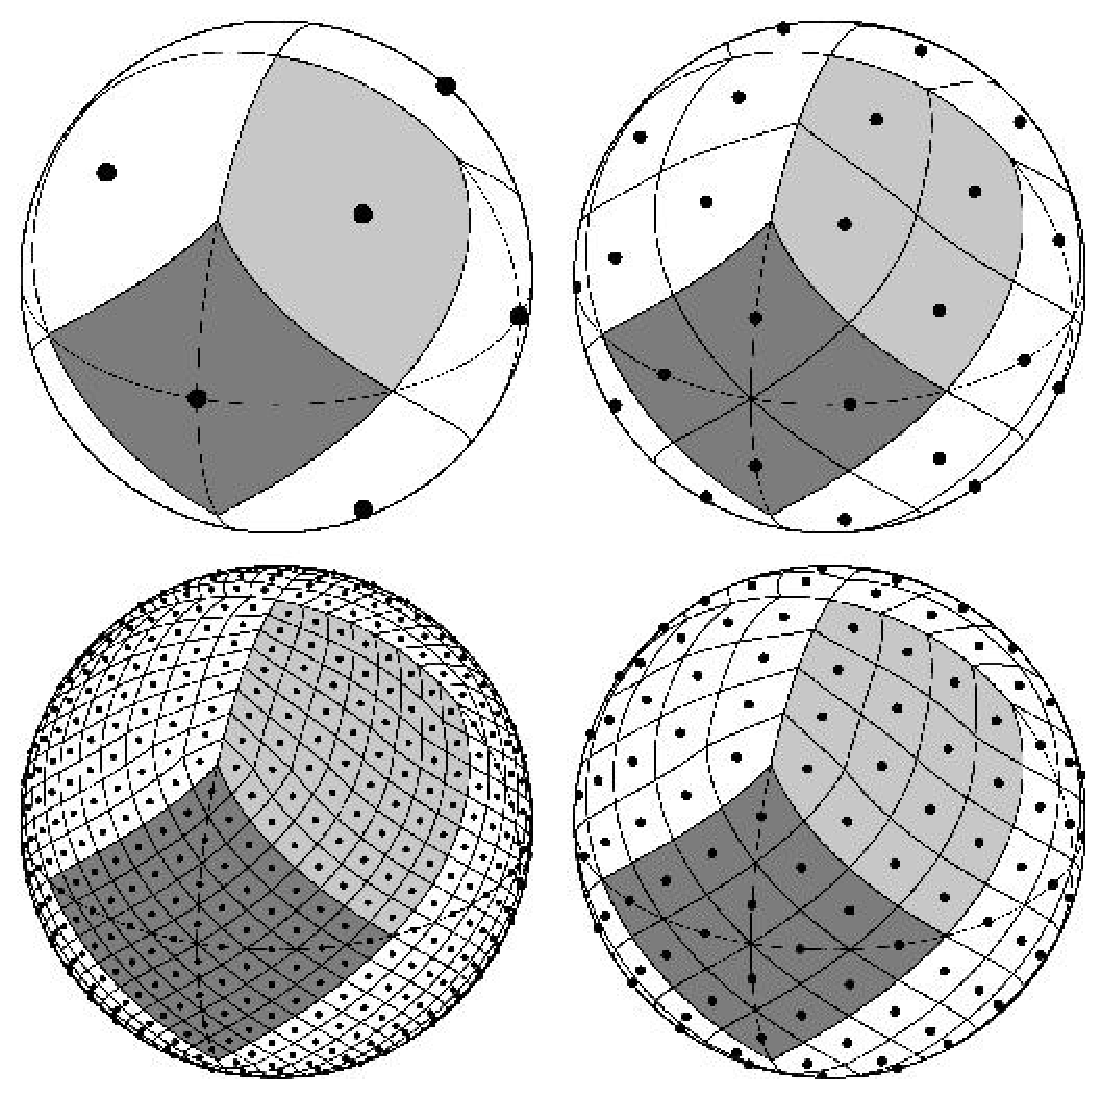
\includegraphics[width=0.5\linewidth]{healpix}}
\caption{Деление сферы на равные по пложади сигменты.}
\label{img:healpix}
\end{figure}

Другим свойством сетки HEALPix является то, что пиксельные центы, представленные черными точками, встречаются на конечном числе колец постоянной широты, количество колец зависит от разрешения сетки HEALPix. Для примера, у зеленогой, желтой, красной и синей сферы их 3, 7, 15, 31 кольцо с постоянной широтой соответственно(?).

Ниже, на рисунке~(\ref{img:cmb}) приведён пример применения HEALPix с высоким разрешением -- Модель реликтового излучения (CMB) (космическое сверхвысокочастотное фоновое излучение), состоящая из 12582912 пикселей (~ 3.4 минут дуги (arcmin)).


\begin{figure}[h]
\begin{minipage}[h]{0.3\linewidth}
\center{
\includegraphics[width=1\linewidth]{exampleCMB} \\На сфере}
\end{minipage}
\hfill
\begin{minipage}[h]{0.69\linewidth}
\center{\includegraphics[width=0.85\linewidth]{Planck-CMB-map-at-high-resolution_planck_cmb_map} \\Проекция Hammer}
\end{minipage}
\caption{Визуализация CMB на HEALPix}
\label{img:cmb}
\end{figure}

\subsection{Распределение разностей паралаксов}\label{sub:smthhealpix}

На рисунках (\ref{img:sf_ra}) (\ref{img:sf_l}) и (\ref{img:sf_lo}), мы видим распределение разностей параллаксов соответственно в экваториальной, галактической и эклиптической системе координат. Заметно, что в эклиптичекой распределение имеет явно симметрийчный, относительно эклиптиеского экватора, характер.

\begin{figure}[h!]
\center{\includegraphics[width=0.5\linewidth]{sf_ra}}
\caption{Среднее распределение модуля параллаксов в экваториальной системе.}
\label{img:sf_ra}
\end{figure}
\begin{figure}[h!]
\center{\includegraphics[width=0.5\linewidth]{sf_l}}
\caption{Среднее распределение модуля параллаксов в галактической системе.}
\label{img:sf_l}
\end{figure}
\begin{figure}[h!]
\center{\includegraphics[width=0.5\linewidth]{sf_lo}}
\caption{Среднее распределение модуля параллаксов в Эклиптической системе.}
\label{img:sf_lo}
\end{figure}

\subsection{Сферические функции}\label{sistem}  
Подтвердить статистическую значимость данной характеристики и отбросить менее сильные мы можем с помощью разложения модуля разностей параллаксов на гармоники сферических функций. Сферические функции широко используются в различных областях математики и физики, их определение можно найти во многих источниках (например, Арфкен, 1970)~\cite{book:arfken}. Впервые  были использованы для анализа систематических разностей положений и собственных движений. Мы впервые используем этот инструмент для анализа систематических разностей параллаксов.
 
Представление модуля разницы параллаксов с помощью линейной комбинации сферических функций можно записать следующим образом.


$$ \Delta_{plx} (l,b) = \sum_{nkp}\delta_{nkp}K_{nkp}(l,b) $$,
где сферические функции имеют вид (Арфкен, 1970)~\cite{book:arfken}.

\begin{equation}\label{f:sf_k}
K_{nkp}(l,b) = R_{nk} \left\{ \begin{array}{ll}
P_{n,0}(b), & \textrm{$k=0, p=1$,}\\
P_{n,k}(b)\sin{kl}, & \textrm{$k\neq0, p=0$,}\\
P_{n,k}(b)\cos{kl}, & \textrm{$k\neq0, p=1$,}
\end{array} \right.
\end{equation}

\begin{equation}
R_{nk} = \sqrt[]{\frac{2n+1}{4\pi}} \left\{ \begin{array}{cc}
\sqrt[]{\frac{2(n-k)!}{(n+k)!}}, & \textrm{$k>0$,}\\
1, & \textrm{$k=0$,}
\end{array} \right.
\end{equation}

В формуле (\ref{f:sf_k}) через $l$ и $b$ обозначены соответственно долгота и широта на сфере, ($0 \leq l \leq 2\pi$; $-\pi/2\leq b \leq \pi/2$); через $P_{nk}(b)$ - полиномы лежандра (при $k = 0$) и присоединенные функции Лежандра (при $k > 0$), которые можно вычислить с помощью следующих рекуррентных соотношений. 
\begin{equation}
\begin{array}{rll}
P_{nk}(b)=&\sin{b\frac{2n-1}{n-k}}P_{n-1,k}(b)-\frac{n+k-1}{n-k}P_{n-2,k}(b), & {}^{k=0,1,...}_{n=k+1,k+2,...}\\
P_{kk}(b)=&\frac{(2k)!}{2^{k}k!}{\cos{b}}^{k}\\
P_{k+1,k}(b)=&\frac{(2k+2)!}{2^{k+1}(k+1)!}{\cos{b}}^{k}\sin{b}
\end{array}
\end{equation}

Для практичности часто вводят линейную нумерацию  сферических коэффициентов $\beta_{nkp}$ и функций $K_{nkp}$ c помощью одного индекса $j$, где

\begin{equation}\label{f:sf_j}
j = n^2 + 2k + p -1
\end{equation}

Каждый может убедиться, что введёные сферические функции удовлетвояют следующим соотношениям:

\begin{equation}
\iint\limits_\Omega \left(K_i \cdot K_j \right) d\omega =  \left\{ \begin{array}{cc}
0, & i \neq j,\\
1, & i = j.
\end{array} \right.
\end{equation}

Иными словами, набор функций $K_{nkp}$ образует на сфере ортонормированную систему функций.




%HealPix имеет два режима разбиения:
%\begin{itemize}
%\item NEST - позволяет работать со сферическими функциями %и не только...

%\item RING - позволяет определять минимальное расстояние до точек и не только...
%\end{itemize}

%\begin{figure}[h]
%\begin{minipage}[h]{0.48\linewidth}
%\center{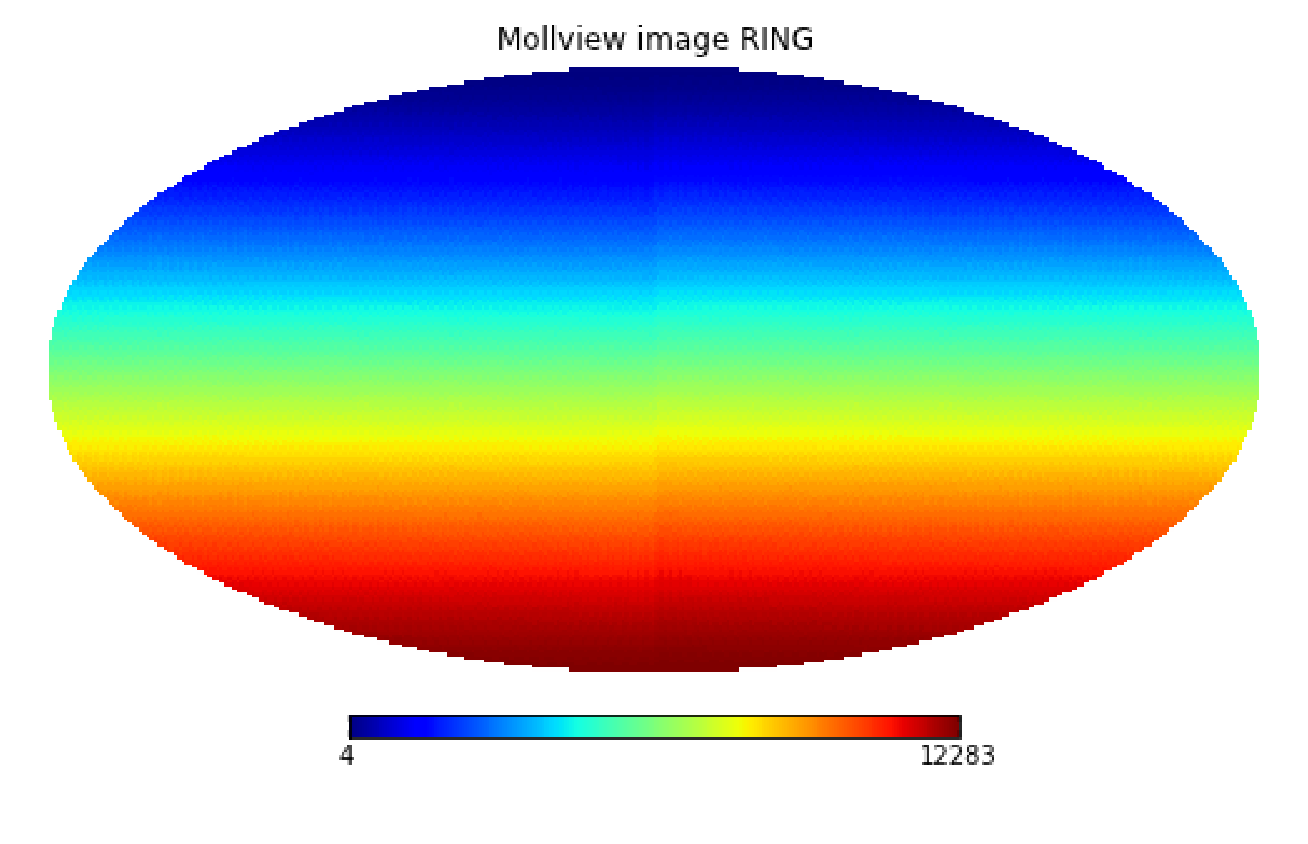
\includegraphics[width=1\linewidth]{moll_nside32_ring}}
%\end{minipage}
%\hfill
%\begin{minipage}[h]{0.48\linewidth}
%\center{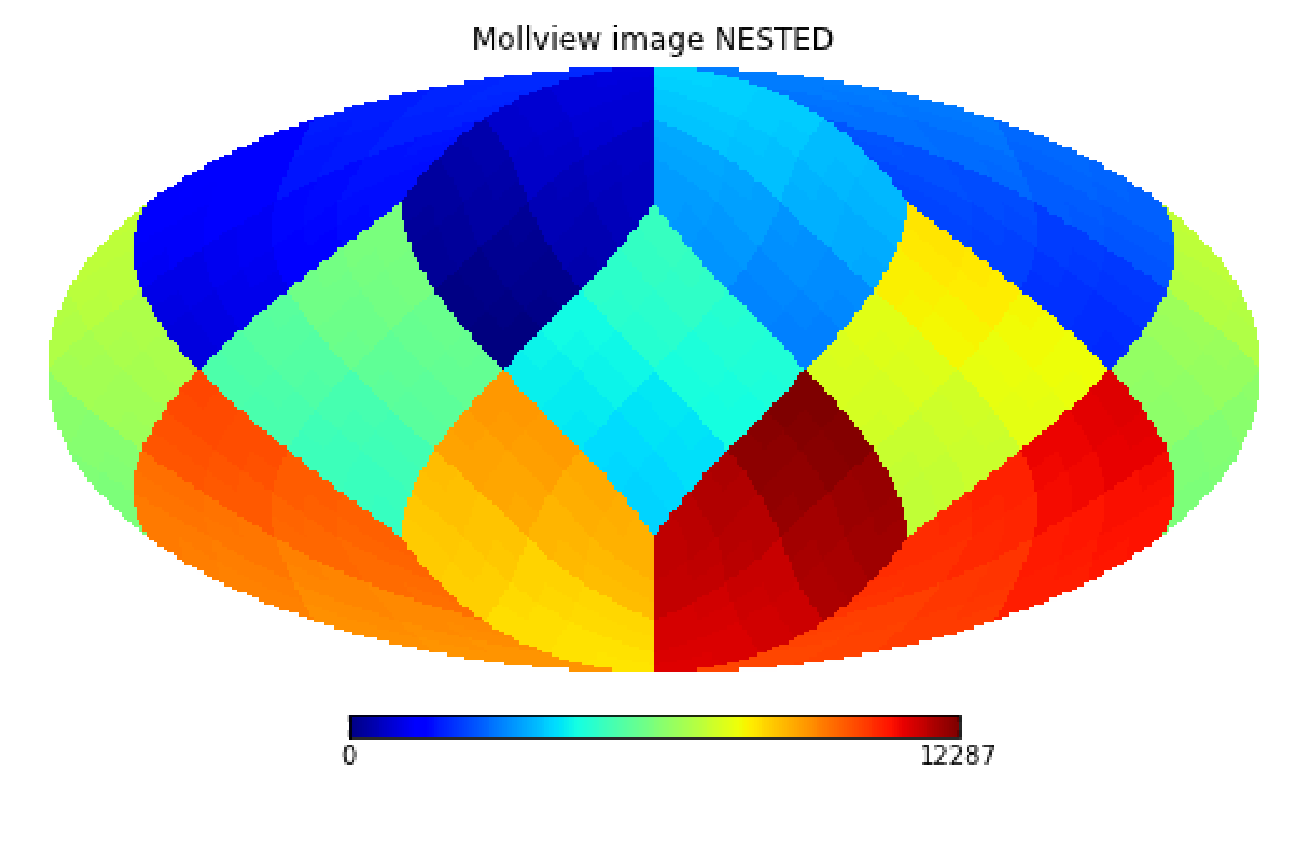
\includegraphics[width=1\linewidth]{moll_nside32_nest}}
%\end{minipage}
%\caption{Пример распределения  пикселей по ring and nest}
%\label{ris:moll_nside32_healpix}
%\end{figure}
%Для нашей задачи отлично подходит NEST.

\subsection{Сферические гармоники}\label{sistem}  
Применив метод Наименьших Квадратов, получили гармоники разложения (Таблица 2). СТоит отметить, что ошибки разложения достаточно малы и сравнимы с незначимыми гармониками: в экватриальной системе координат - 0.030270, галактической - 0.0308442 и эклиптической - 0.0300682.

\begin{table}[h!]
\centering
\caption{Сферические гармоники в экваториальной, галактической и эклиптической сисмете со стандартными отклонениями для этих же систем, соответственно}
\label{tabular:tgas_st}
\begin{tabular}{c|c|c|c|c|c|c}
%\rowcolor{Gray} 
\hline 	
$j$ &$\beta_{J_{ra,dec}}$ &$\beta_{J_{l,b}}$ &$\beta_{J_{lon,lat}}$ &$\sigma_{ra,dec}$ &$\sigma_{l,b}$ & $\sigma_{lon,lat}$\\
\hline 	
\rowcolor{Gray}
0 &3.855 &3.857 &3.856 &0.554 &0.5505 &0.5541\\
1 &-0.017 &-0.022 &0.002 &0.554 &0.5505 &0.5541\\
2 &0.044 &-0.023 &0.048 &0.554 &0.5505 &0.5541\\
3 &-0.024 &-0.046 &-0.026 &0.554 &0.5505 &0.5541\\
\rowcolor{Gray}
4 &-0.382 &0.148 &-0.554 &0.554 &0.5505 &0.5541\\
5 &-0.397 &0.316 &-0.049 &0.554 &0.5505 &0.5541\\
6 &0.092 &-0.088 &0.137 &0.554 &0.5505 &0.5541\\
7 &0.137 &0.01 &0.091 &0.554 &0.5505 &0.5541\\
8 &0.06 &0.451 &-0.035 &0.554 &0.5505 &0.5541\\
9 &0.005 &0.019 &0.007 &0.554 &0.5505 &0.5541\\
10 &0.002 &-0.024 &-0.009 &0.554 &0.5505 &0.5541\\
11 &0.045 &0.022 &0.037 &0.554 &0.5505 &0.5541\\
12 &0.011 &-0.027 &-0.029 &0.554 &0.5505 &0.5541\\
13 &0.006 &-0.024 &0.008 &0.554 &0.5505 &0.5541\\
14 &0.006 &-0.017 &0.0 &0.554 &0.5505 &0.5541\\
15 &0.033 &0.011 &0.024 &0.554 &0.5505 &0.5541\\
16 &-0.02 &0.034 &-0.087 &0.554 &0.5505 &0.5541\\
17 &-0.056 &-0.063 &-0.042 &0.554 &0.5505 &0.5541\\
18 &-0.022 &0.011 &-0.048 &0.554 &0.5505 &0.5541\\
19 &-0.039 &0.027 &-0.022 &0.554 &0.5505 &0.5541\\
20 &0.064 &0.088 &0.057 &0.554 &0.5505 &0.5541\\
21 &0.058 &-0.054 &0.044 &0.554 &0.5505 &0.5541\\
22 &0.05 &-0.065 &-0.015 &0.554 &0.5505 &0.5541\\
23 &-0.049 &-0.021 &-0.063 &0.554 &0.5505 &0.5541\\
24 &-0.071 &0.016 &-0.043 &0.554 &0.5505 &0.5541\\
25 &0.021 &-0.053 &0.006 &0.554 &0.5505 &0.5541\\
26 &0.004 &0.02 &-0.016 &0.554 &0.5505 &0.5541\\
27 &0.001 &-0.035 &0.014 &0.554 &0.5505 &0.5541\\
28 &-0.012 &0.016 &0.019 &0.554 &0.5505 &0.5541\\
29 &0.015 &0.039 &-0.026 &0.554 &0.5505 &0.5541\\
30 &-0.042 &0.006 &-0.008 &0.554 &0.5505 &0.5541\\
31 &-0.036 &0.009 &-0.018 &0.554 &0.5505 &0.5541\\
32 &-0.024 &-0.01 &0.037 &0.554 &0.5505 &0.5541\\
33 &-0.016 &-0.004 &-0.046 &0.554 &0.5505 &0.5541\\
34 &-0.013 &0.033 &0.009 &0.554 &0.5505 &0.5541\\
35 &-0.04 &0.02 &-0.036 &0.554 &0.5505 &0.5541\\
36 &-0.028 &0.025 &0.021 &0.554 &0.5505 &0.5541\\
\end{tabular}
\end{table}

Как мы видим из таблици, все системы имеют значимые нулевые гармоники, в 8 раз превосходящие самую ближайшую гармонику. Так же в эклиптической системе координат присутствует 4 гармоника, чуть больше отдалённая от среднего, чем дисперсия. 

Нулевая гармоника -- константа, она нам никак не можможет  для статистичегоского анализа. 

\begin{figure}[h!]
\center{\includegraphics[width=0.5\linewidth]{sfff}}
\caption{Значимые гармоники в сферической еклиптической системе}
\label{img:sfff}
\end{figure}

На рисунке (\ref{img:nobs}) видно, что модуль разности паралаксов  у полюсов меньше, чем на экваторе, это объясняется законом вращения аппарата Hipparcos - чем чаще он наблюдал звезду,
тем точнее у нее вычислялся параллакс в XHIP, и тем ближе значение параллакса оказался к значениям паралакса для этого же объекта из TGAS.


\begin{figure}[h!]
\center{\includegraphics[width=0.5\linewidth]{nobs}}
\caption{Колличество наблюдений определённых областей аппаратом hipparcos.\\Там где синий - меньше всего наблюдали и соответственно больше ошибок, и противоположная ситуация у полюсов.}
\label{img:nobs}
\end{figure}

%\begin{table}[h!]
%\centering
%\caption{Общая статистика по параллаксам и их ошибкам в каталоге TGAS}
%\label{tabular:tgas_st}
%\begin{tabular}{c|c|c}
%\rowcolor{Gray} 
%{}&parallax &parallax error\\
%\hline 	
%count &2057050	&2057050\\
%mean	&2.477627e+00	&3.850052e-01\\
%std	&2.910183e+00	&1.699272e-01\\
%min	&-2.481995e+01	&2.039740e-01\\
%25\%	&1.030510e+00	&2.681603e-01\\
%50\%	&1.780198e+00	&3.220124e-01\\
%75\%	&3.015706e+00	&4.360010e-01\\
%max	&2.958036e+02	&9.999985e-01\\
%\end{tabular}
%\end{table}


\section{Заключение}\label{conclusion}
В ходе решения задач было разработано программное обеспечение для работы с каталогом TGAS и XHIP, визуализации данных и разложения на сферические гармоники. Были получены коэффициенты разложения в сферические функции для различных раборов данных в разных Небесных сферах. (Раздел 4.2).
Данная работа носит подготовительный характер для обработки последующих релизов каталога Gaia, в том числе релиза Gaia
Data Release 2, вышедшего 25 апреля 2018 года. В новой версии каталога значитель-но увеличилось число объектов, для которых известны пять астрометри-ческих параметров.

\newpage
\section{Список использованной литературы}\label{conclusionlit}
%\bibliographystyle{unsrt}
%\bibliography{kursach.bib}
\printbibliography[type=online,title={Сайты}]
\printbibliography[type=book,title={Статьи:}]


\appendix

\section*{Приложение}

\newpage
\begin{landscape}
\begin{spacing}{1.0}
%\rotatebox{90}{ %это обеспечивает поворот любого объекта
%\begin{minipage}{1.6\linewidth}
\begin{table}[h]
\caption{Рекордсмены по разности параллаксов}
\label{tabular:75_25}
\begin{tabular}{|r|r|r|r|r|r|r|r|}
\hline 	
$hip_{id}$ &$\pi_{tgas}$ &$\pi_{hip}$ &$\pi_{difference}$ &$\pi_{difference_{abs}}$ &$\pi_{error_{tgas}}$ &$\pi_{error_{hip}}$ &$n_{obs_{hip}}$\\
\hline 
21000&3.6135194843037333&93.67&90.05648051569626&90.05648051569626&0.43092538640597655&7.62&41\\
42525&5.939340804931861&68.54&62.60065919506815&62.60065919506815&0.4989712380569283&15.51&88\\
117081&7.767833345528349&63.56&55.79216665447166&55.79216665447166&0.391415724958141&21.02&52\\
92059&1.0253014604321609&55.49&54.46469853956784&54.46469853956784&0.2575126107035069&13.48&74\\
16582&3.3525394898163663&46.79&43.43746051018363&43.43746051018363&0.3379833330672927&47.48&78\\
49971&10.032882741927454&53.21&43.17711725807255&43.17711725807255&0.2739555697690759&17.78&79\\
14101&148.51025482141657&106.16&-42.35025482141657&42.35025482141657&0.9418350466246392&16.51&95\\
90368&9.239325596436997&51.0&41.760674403563&41.760674403563&0.2380419233789036&10.37&128\\
87784&0.9016399080820414&41.3&40.398360091917965&40.398360091917965&0.2617397591615193&8.36&266\\
11167&1.6005219496065075&40.32&38.71947805039349&38.71947805039349&0.36195791278945777&18.63&146\\
17468&3.6968394746639017&41.4&37.703160525336095&37.703160525336095&0.9324727968205918&15.72&62\\
26690&6.758462929784543&43.01&36.251537070215456&36.251537070215456&0.2790695120679915&28.39&55\\
63028&6.593468516719788&41.33&34.73653148328021&34.73653148328021&0.38054460916425065&10.0&140\\
2715&8.99457132952772&43.6&34.605428670472286&34.605428670472286&0.36759122490605495&15.16&73\\
43650&1.8692458424123573&36.4&34.530754157587644&34.530754157587644&0.2636490611144113&8.77&131\\
37103&1.177487047842296&33.63&32.452512952157704&32.452512952157704&0.23851513809910355&20.31&52\\
8356&1.875554375591414&33.99&32.11444562440859&32.11444562440859&0.3490448951334293&20.35&89\\
33404&1.6814129603685233&33.48&31.798587039631478&31.798587039631478&0.2728863787154474&16.3&261\\
35873&1.7659760403953777&32.58&30.814023959604626&30.814023959604626&0.3144475734924109&11.18&84\\
109335&3.5040942969592948&34.06&30.55590570304071&30.55590570304071&0.2418385213119765&8.86&123\\
109930&2.941969216919245&32.96&30.018030783080764&30.018030783080764&0.23828269976331&12.73&127\\
26111&0.8614923854606678&30.22&29.358507614539327&29.358507614539327&0.2734412733226204&1.94&247\\
99720&6.2138396569790295&35.41&29.196160343020967&29.196160343020967&0.4081948331799583&9.14&84\\
26462&7.749974783835219&36.88&29.130025216164785&29.130025216164785&0.2542881333731009&15.57&94\\
86685&2.5910519158726935&30.58&27.98894808412731&27.98894808412731&0.22941196532598346&14.02&62\\
\hline 
\end{tabular}
\end{table}

\newpage

\begin{table}[h]
\caption{Рекордсмены по разности параллаксов}
\label{tabular:75_50}
\begin{tabular}{|r|r|r|r|r|r|r|r|}
\hline 	
$hip_{id}$ &$\pi_{tgas}$ &$\pi_{hip}$ &$\pi_{difference}$ &$\pi_{difference_{abs}}$ &$\pi_{error_{tgas}}$ &$\pi_{error_{hip}}$ &$n_{obs_{hip}}$\\
\hline 
101453&0.47229964249774603&27.73&27.25770035750225&27.25770035750225&0.3815522125350718&22.97&72\\
80365&0.3252566015932853&27.29&26.964743398406714&26.964743398406714&0.2991317461151089&17.1&105\\
570&2.286728392538792&28.95&26.66327160746121&26.66327160746121&0.29479727936398475&12.23&116\\
66125&29.328255835837076&55.78&26.45174416416293&26.45174416416293&0.28838700860065314&10.02&142\\
91557&56.48334976858664&30.49&-25.993349768586643&25.993349768586643&0.26665022041629555&7.89&71\\
100625&2.6086537349321026&27.99&25.381346265067897&25.381346265067897&0.4762157223925944&7.06&88\\
111276&4.355962433196507&29.73&25.374037566803487&25.374037566803487&0.2491454760570632&7.24&106\\
47645&31.714569962446753&6.92&-24.79456996244675&24.79456996244675&0.5027812716747218&4.05&97\\
47846&2.0769676160399926&26.74&24.663032383960005&24.663032383960005&0.3718433605661264&13.43&119\\
96643&6.704986888643228&31.35&24.645013111356768&24.645013111356768&0.6719925058062542&10.99&86\\
64289&5.528102793567756&30.02&24.491897206432238&24.491897206432238&0.2729570135141233&12.06&216\\
46637&28.667826266554712&52.99&24.322173733445286&24.322173733445286&0.3057977692475484&13.11&62\\
14137&15.784241966318724&39.87&24.085758033681273&24.085758033681273&0.9159903829184022&10.61&114\\
31998&1.4152700481213487&24.89&23.474729951878647&23.474729951878647&0.3038217166099563&8.85&105\\
74143&4.583228557144263&27.83&23.24677144285573&23.24677144285573&0.2362874545789483&14.7&53\\
47839&17.35715805587964&40.16&22.80284194412036&22.80284194412036&0.2874781695636456&7.14&143\\
7739&0.5226712293088758&22.68&22.157328770691123&22.157328770691123&0.4886794246222954&11.61&139\\
7197&5.962195894692861&27.71&21.74780410530714&21.74780410530714&0.2822776116397612&7.8&152\\
68158&1.0248438291894155&22.71&21.685156170810586&21.685156170810586&0.25628523607246856&9.75&93\\
5669&5.099146141909381&25.94&20.840853858090615&20.840853858090615&0.5073643719931885&15.48&56\\
70446&10.257532551168296&30.89&20.632467448831704&20.632467448831704&0.2638598628788957&10.84&140\\
91154&26.083310925789466&46.71&20.62668907421053&20.62668907421053&0.7623642510543536&1.44&80\\
95652&5.5940400684495994&25.56&19.965959931550397&19.965959931550397&0.3290609310114135&13.67&113\\
93722&0.44814565033275344&20.39&19.941854349667246&19.941854349667246&0.29492235794973065&10.76&122\\
58241&28.22518406478849&8.35&-19.87518406478849&19.87518406478849&0.2582119869663121&10.74&86\\
\hline 
\end{tabular}
\end{table}

\newpage

\begin{table}[h]
\caption{Рекордсмены по разности параллаксов}
\label{tabular:75_75}
\begin{tabular}{|r|r|r|r|r|r|r|r|}
\hline 	
$hip_{id}$ &$\pi_{tgas}$ &$\pi_{hip}$ &$\pi_{difference}$ &$\pi_{difference_{abs}}$ &$\pi_{error_{tgas}}$ &$\pi_{error_{hip}}$ &$n_{obs_{hip}}$\\
\hline 
10332&0.5496683653487973&20.29&19.7403316346512&19.7403316346512&0.34515024281556256&9.42&118\\
41955&7.370182159796287&26.92&19.549817840203715&19.549817840203715&0.2421192538511551&5.33&149\\
58988&0.8162321311506745&19.89&19.073767868849327&19.073767868849327&0.3197442591937322&12.5&140\\
42652&3.256530578152378&22.11&18.85346942184762&18.85346942184762&0.2298275358550482&5.91&189\\
75262&4.753556800163254&23.58&18.826443199836746&18.826443199836746&0.2326450723449282&9.0&63\\
15691&5.67209516705868&24.15&18.47790483294132&18.47790483294132&0.2283915861455185&11.63&183\\
66077&59.9278117924246&78.37&18.442188207575406&18.442188207575406&0.5397605666370869&19.88&125\\
100179&3.2465325232423234&21.57&18.323467476757678&18.323467476757678&0.2320522094008197&4.39&94\\
62830&4.197567674413529&22.27&18.07243232558647&18.07243232558647&0.3354698950878142&12.19&65\\
72481&21.560864630663342&3.86&-17.700864630663347&17.700864630663347&0.550561071487674&1.21&161\\
67693&2.7795586772228105&20.45&17.670441322777194&17.670441322777194&0.37833586991304&11.83&125\\
16983&2.3114210871896863&19.47&17.158578912810313&17.158578912810313&0.3219764548866185&16.07&63\\
81696&0.8500613651480577&17.95&17.099938634851938&17.099938634851938&0.35976853683275084&16.68&51\\
80381&34.10435762053698&51.0&16.89564237946302&16.89564237946302&0.2721318847333499&5.18&91\\
105041&18.72045277115448&1.97&-16.750452771154478&16.750452771154478&0.3218370441623262&9.72&78\\
47836&17.45983396904449&33.9&16.44016603095551&16.44016603095551&0.2858313610117272&14.14&143\\
97232&1.1057765415995844&17.5&16.394223458400415&16.394223458400415&0.6357870352980504&5.66&138\\
8181&4.4856992038002526&20.59&16.104300796199748&16.104300796199748&0.2820151130234709&12.95&81\\
16064&2.241531209436262&18.3&16.05846879056374&16.05846879056374&0.3048204876440345&7.14&110\\
95579&0.6979718456231865&16.56&15.862028154376812&15.862028154376812&0.3549002292665109&6.95&89\\
30550&17.475212996728608&1.62&-15.855212996728609&15.855212996728609&0.24626716274819915&4.76&94\\
108066&3.574489184181695&19.27&15.695510815818306&15.695510815818306&0.2799130292658689&12.33&56\\
1512&18.674652360947487&3.05&-15.624652360947485&15.624652360947485&0.6081619588077191&3.0&118\\
50618&2.983022260996149&18.6&15.616977739003852&15.616977739003852&0.2579682795408065&13.05&135\\
111932&23.650711066538488&39.03&15.379288933461511&15.379288933461511&0.34570068330938913&12.07&79\\
\hline 
\end{tabular}
\end{table}

\end{spacing}
\end{landscape}
\newpage

\end{document}
